\documentclass[a0paper,landscape, fontscale=0.4]{baposter}

\usepackage{graphicx} % Required for including images
\graphicspath{{figures/}} % Directory in which figures are stored
\usepackage{qrcode} % For creating QR codes

\usepackage{fix-cm} % Arbitrary font size

\renewcommand{\familydefault}{\sfdefault}
\usepackage{avant}

\usepackage{amsmath} % For typesetting math

\selectcolormodel{HTML}
\definecolor{oistred}{HTML}{C80019} % Defines the color used for content box headers
\definecolor{grey}{rgb}{0.06, 0.05, 0.03}

\begin{document}

\begin{poster}{ columns=5,
headerborder=closed, % Adds a border around the header of content boxes
colspacing=1em, % Column spacing
bgColorOne=white, % Background color for the gradient on the left side of the poster
bgColorTwo=white, % Background color for the gradient on the right side of the poster
borderColor=oistred, % Border color
headerColorOne=white, % Background color for the header in the content boxes (left side)
headerColorTwo=oistred, % Background color for the header in the content boxes (right side)
headerFontColor=grey, % Text color for the header text in the content boxes
boxshade= plain,
boxColorOne=white, % Background color of the content boxes
textborder=roundedleft, % Format of the border around content boxes, can be: none, bars, coils, triangles, rectangle, rounded, roundedsmall, roundedright or faded
eyecatcher=true, % Set to false for ignoring the left logo in the title and move the title left
headerheight=0.01 \textheight, % Height of the header
headershape=roundedright, % Specify the rounded corner in the content box headers, can be: rectangle, small-rounded, roundedright, roundedleft or rounded
headerfont=\Large\bf\textsc, % Large, bold and sans serif font in the headers of content boxes
%textfont={\setlength{\parindent}{1.5em}}, % Uncomment for paragraph indentation
linewidth=2pt % Width of the border lines around content boxes
 } {} {}


% Center message
\begin{posterbox}[
    name = message,  % Name for alignment 
    column = 1, % Second column 
    span = 3, % Over 3 columns
    boxColorOne=oistred, % Changing background color
    headershade=plain,  % Changing header style
    headerColorOne=oistred % Changing header color
    ]{}
    \fontsize{45}{50} \selectfont  \color{white} % Changing font size and color
    
    % Adjust vertical and horizontal spaces as you like
    \vspace{2em} 
    
    \hspace{1em}
    \begin{minipage}[c][ 0.5 \textheight ]{0.6\textwidth}

        We generate a \textbf{formal representation} of all possible \textbf{states} and \textbf{state transitions} of AI \textbf{agents interacting} on a \textbf{grid}

        \vspace{2em}
        
        \LARGE 
        Tom Burns and Robert Tang\\ OIST Graduate University, Japan
    \end{minipage}

    
    % Generating the QR code. Alternatively, they can be generated online with tools such as https://www.qrcode-monkey.com
    \hfill 
    \colorbox{white}{ \makebox[4.7em]{
        \color{black} 
        \qrcode[height = 4em,padding]{https://tfburns.com} }
    } \hspace{0.3em}
    
    \vspace{1em}
    
    \hfill {\normalsize tfburns.com | thomas.burns@oist.jp | +81 (0)90 6863 7039 } \hspace{0.3em}
    
     \vspace{-2.6em}
     
\includegraphics[width=\textwidth, trim= 3 8 3 0]{footer-white.png}
\end{posterbox}

\begin{posterbox}[name=abstract,column=0,row=0]{Abstract}

Gridworlds are a popular and powerful test-bed for artificial intelligence (AI) algorithms, especially in reinforcement learning and associated AI safety problems. To describe how AI agents behave in such gridworlds, we consider gridworlds as reconfigurable systems and construct their state complexes. These state complexes reveal the underlying structures and patterns in the system's possible reconfigurations. This work incorporates the concepts of gridworlds, reconfigurable systems, and state complexes to show structures and patterns found in the state complexes of example gridworlds.
\end{posterbox}

\begin{posterbox}[name=grid,below=abstract]{Gridworlds}
\begin{center}
    \quad \tikz\draw[green,fill=green] (0,0) circle (.5ex); agent
    \quad \tikz\draw[blue,fill=blue] (0,0) circle (.5ex); object
    \quad \tikz\draw[gray,fill=gray] (0,0) circle (.5ex); floor
    \quad \tikz\draw[black,fill=white] (0,0) circle (.5ex); wall
    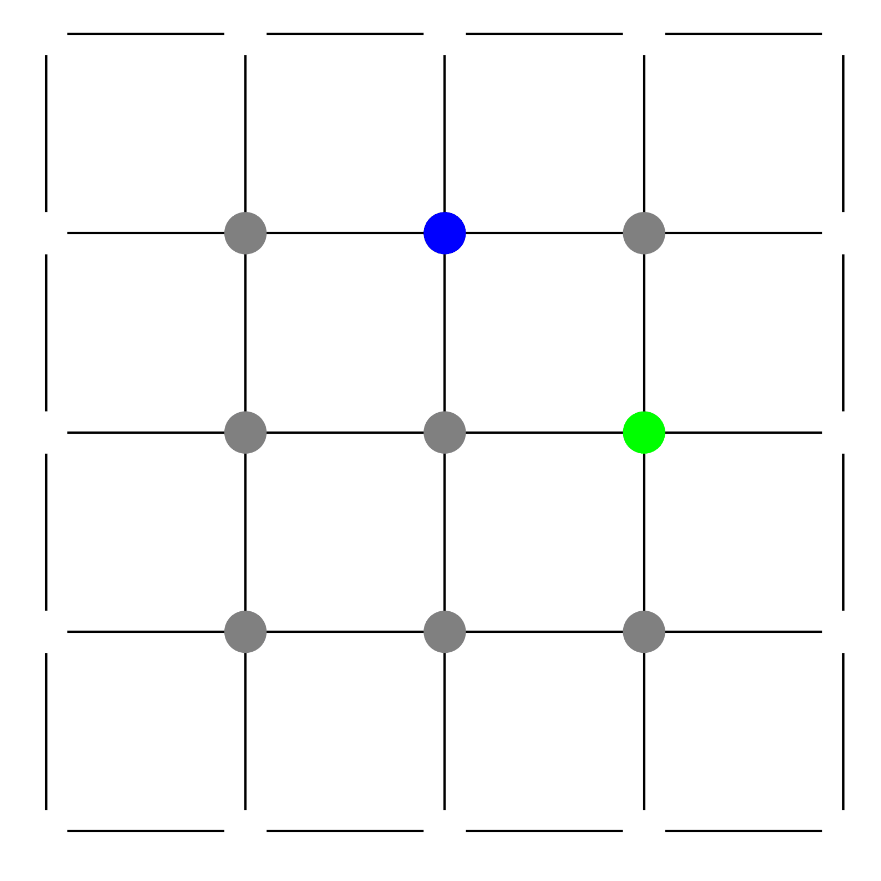
\includegraphics[height=10em]{petal-walk-1-world-crop.png}
\end{center}

Gridworlds are simplified, grid-like environments in which each \textit{cell} of the grid may be assigned a \textit{label}. In the example above, these labels are \textcolor{green}{agent}, \textcolor{blue}{object}, \textcolor{gray}{floor}, and wall. Such environments can be used to test and develop AI algorithms, particularly in reinforcement learning \cite{Leike:2017}.
\end{posterbox}



\begin{posterbox}[name=reconfigsys,below=grid]{Reconfigurable systems}

Ghrist \& Peterson \cite{Ghrist-Peterson:2007} define reconfigurable systems as a collection of labels on a graph, where local rearrangements of the labels represent reconfigurations of the system.
\vspace{0.15cm}

From \cite{Ghrist-Peterson:2007}: $G$ is a graph. $A$ is a set of possible labels on the vertices of $G$.

A \textit{generator} $\phi$ is a collection of three objects:
\begin{itemize}
    \item the \textit{support}, $SUP(\phi) \subset G$
    \item the \textit{trace}, $TR(\phi) \subset SUP(\phi)$
    \item a \textit{relabelling} for the vertex set $TR(\phi)$
\end{itemize}
\end{posterbox}



\begin{posterbox}[name=scs,below=reconfigsys,bottomaligned=message]{State Complexes}
\begin{center}
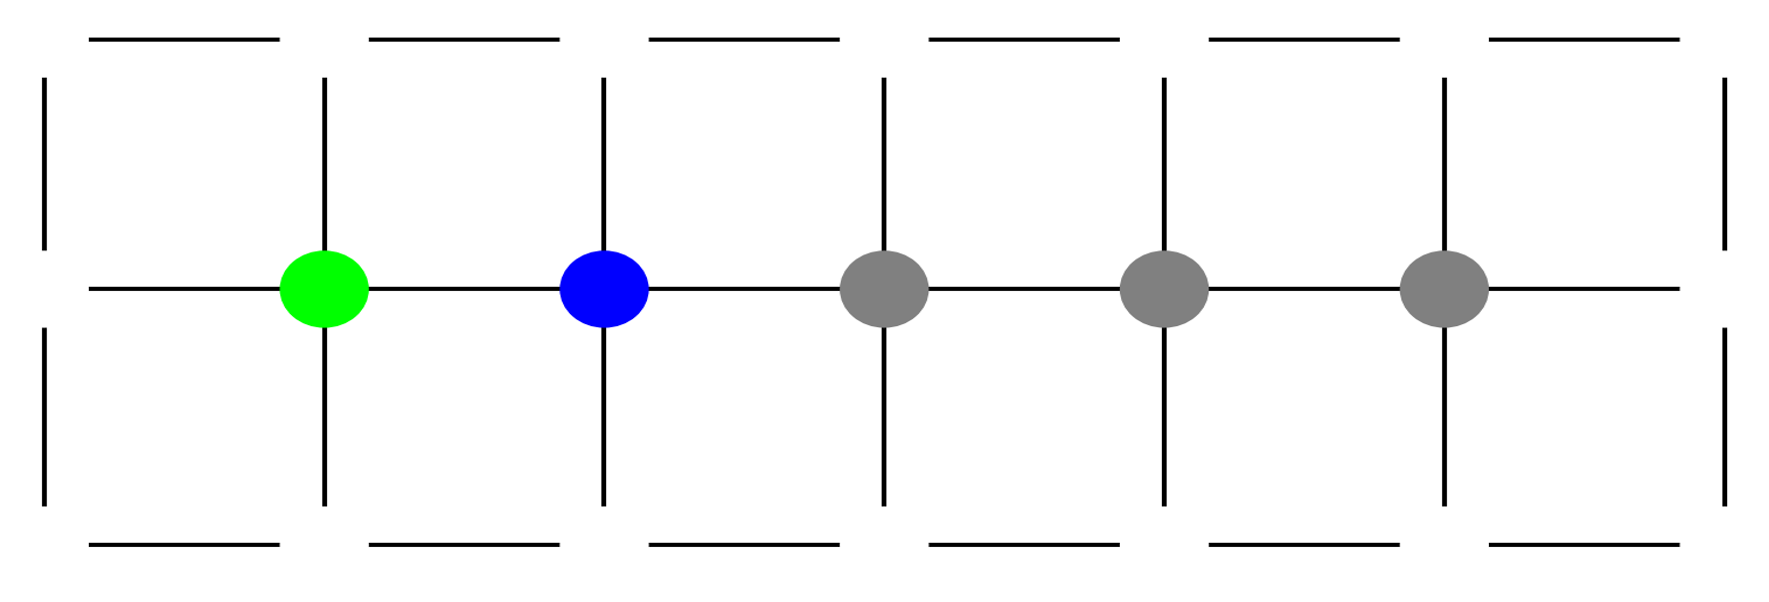
\includegraphics[width=0.7\textwidth]{coorridor.PNG}
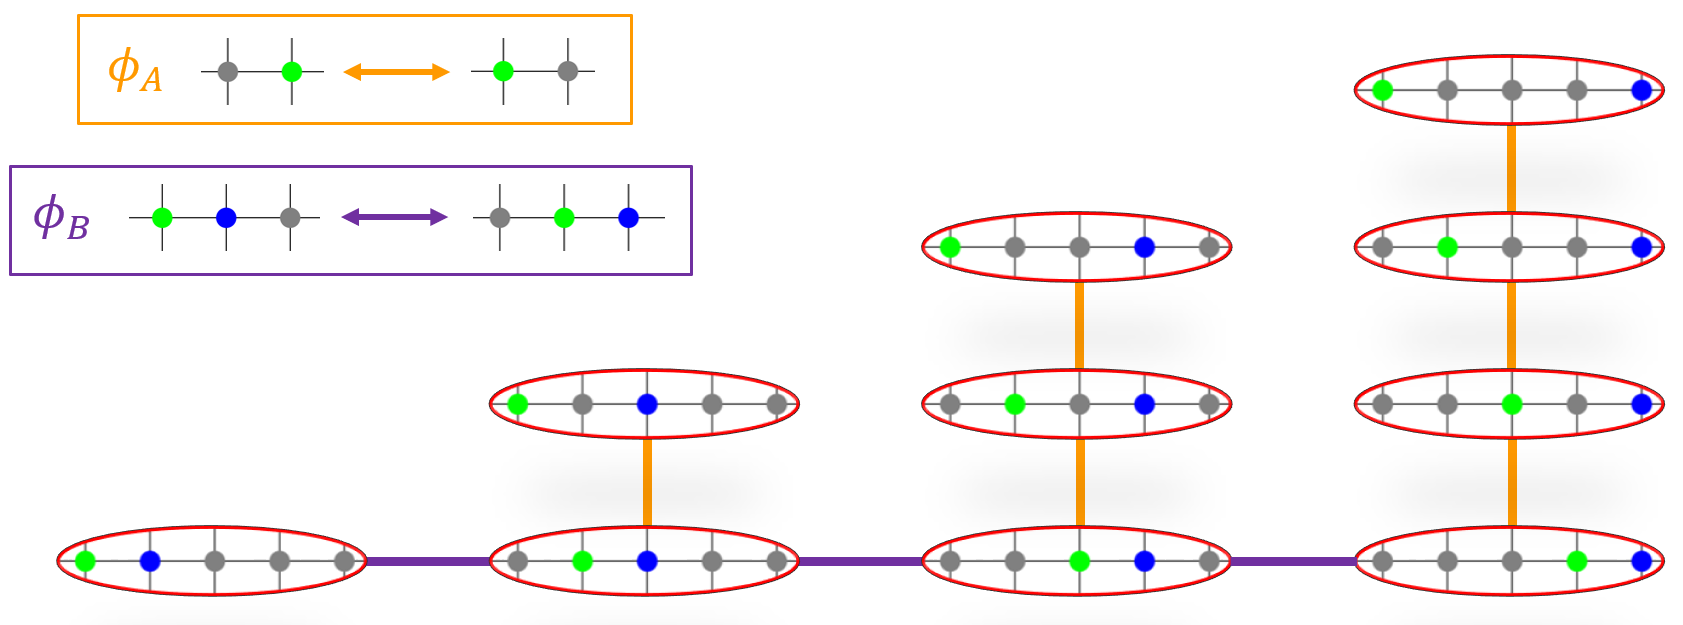
\includegraphics[width=0.8\textwidth]{SC-example.PNG}
\end{center}

Ghrist \& Peterson \cite{Ghrist-Peterson:2007} define a \textcolor{red}{state} of a reconfigurable system as a choice of labels (chosen from $A$) for every vertex of $G$.
\vspace{0.15cm}
$$\textcolor{red}{s_i}:V(G) \rightarrow A$$
The state complex $S$ is a graph with vertices corresponding to states, with edges connecting a pair states differing by a single generator.
\end{posterbox}



\begin{posterbox}[name=scsofgrids,column=4]{S.C.s of Gridworlds}
\begin{center}
    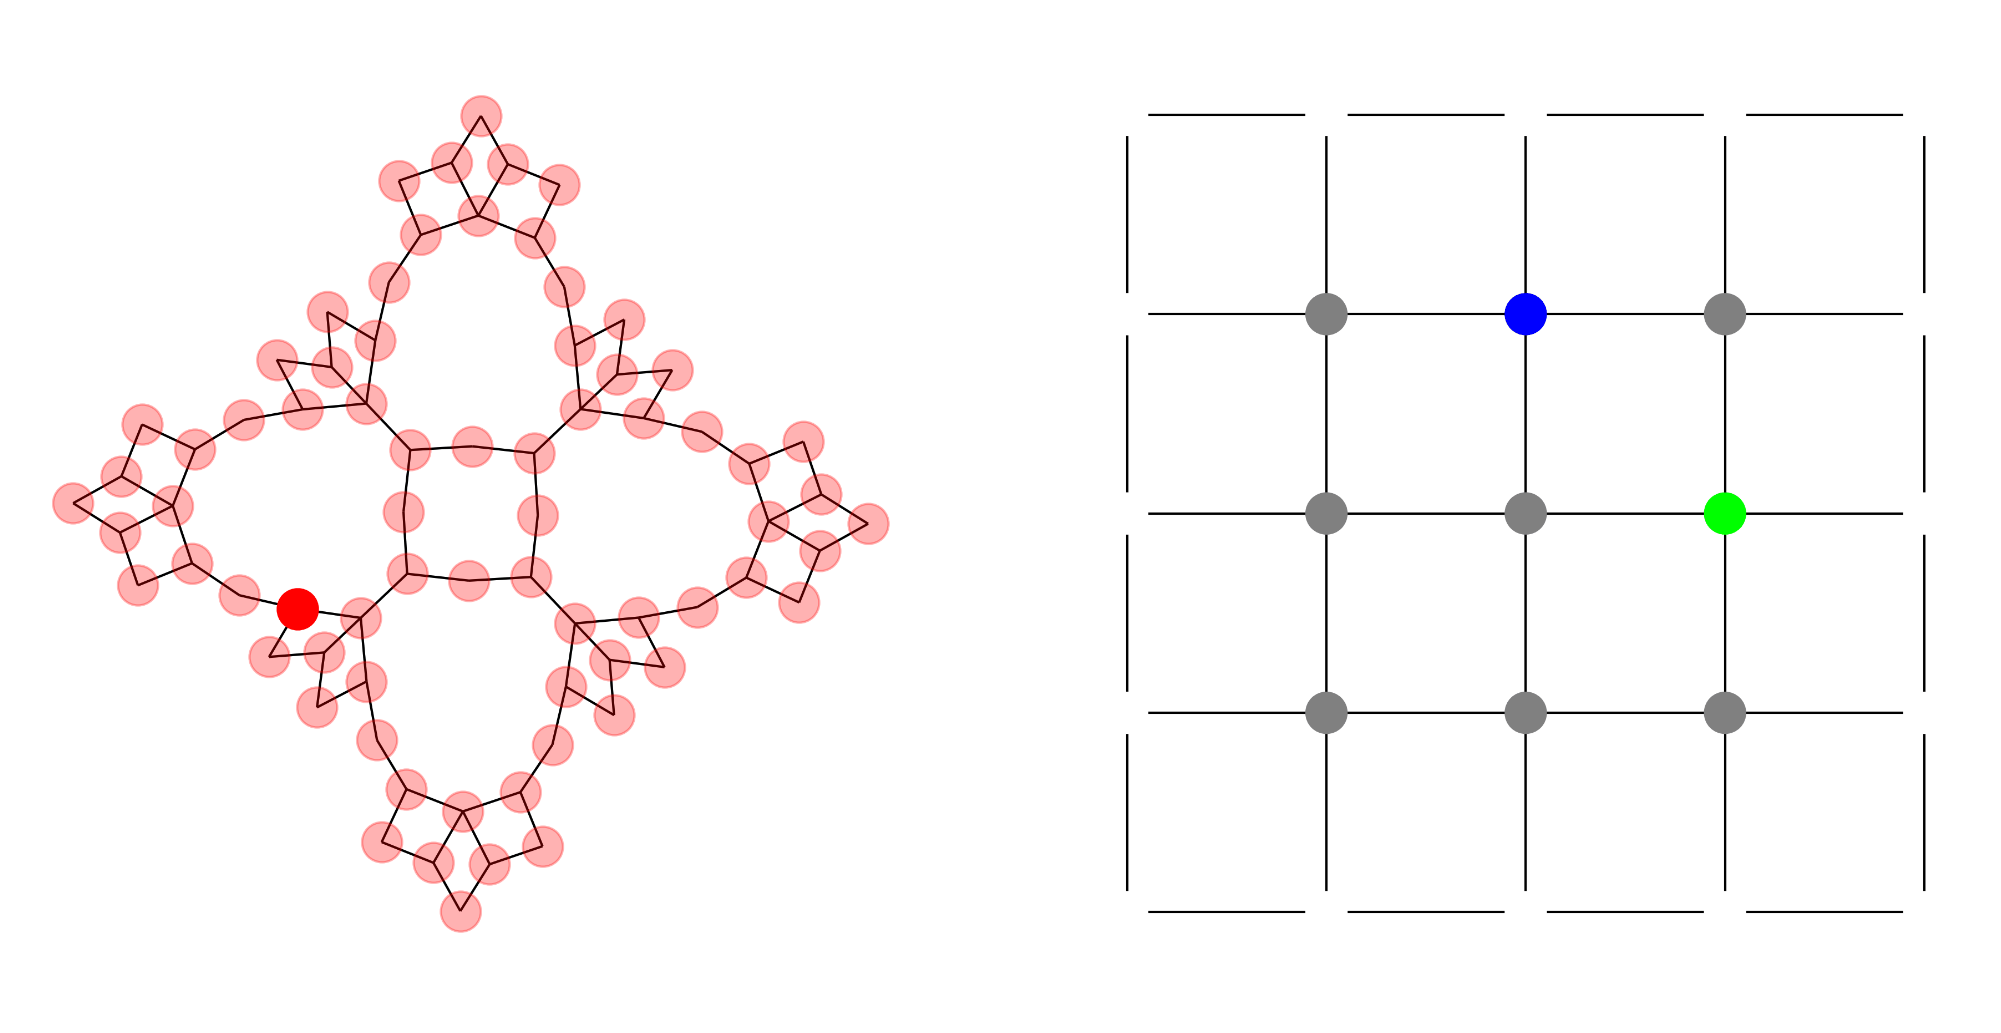
\includegraphics[width=1\textwidth]{petal-walk-1.PNG}
\end{center}

State complexes often capture symmetries in a gridworlds' geometry or labelling, as shown in these examples. The petal-like state complex above shows different scales of geometry; for each position of the \textcolor{blue}{object} there exists a subgraph of 8 verticies (representing the 8 possible locations of the \textcolor{green}{agent}) which is connected to as many other subgraphs as is possible for the \textcolor{green}{agent} to push or pull the \textcolor{blue}{object} to a different location from the current location represented in that subgraph.

\vspace{0.6cm}
\begin{center}
    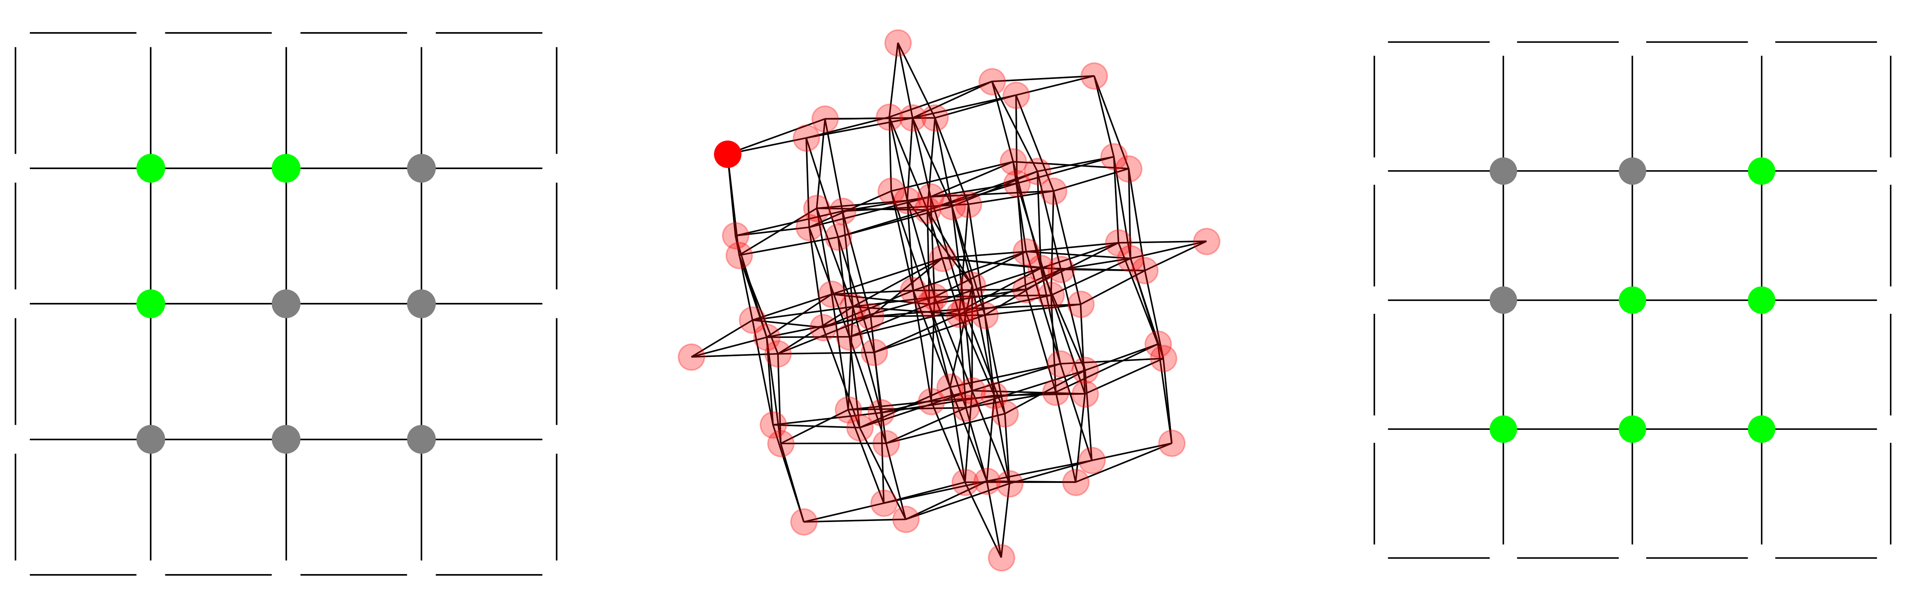
\includegraphics[width=1\textwidth]{3-6-agents.PNG}
\end{center}

We also find that some state complexes are subgraphs of others.

\vspace{0.2cm}
\begin{center}
    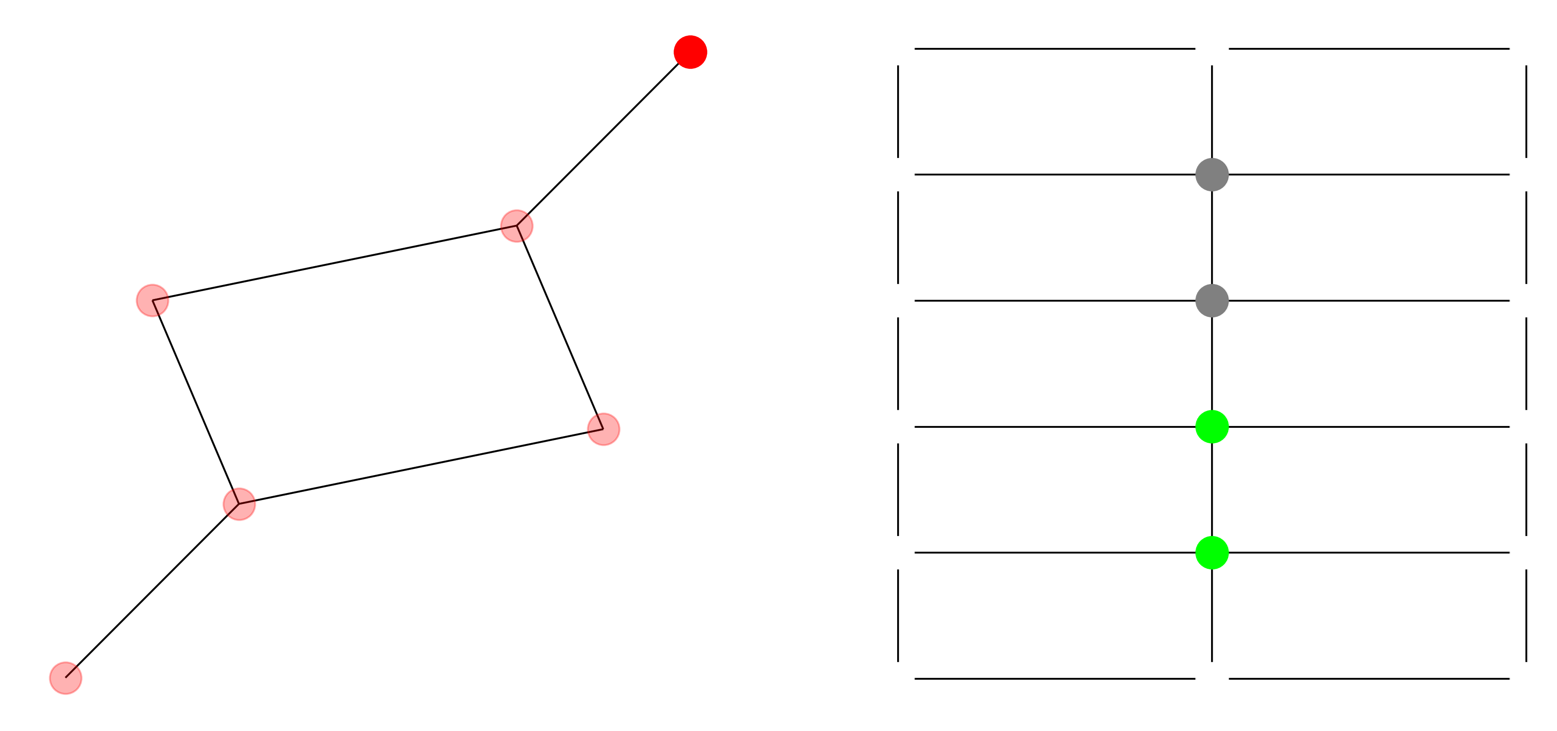
\includegraphics[width=0.6\textwidth]{corridor-2.PNG}
    \vspace{0.2cm}
    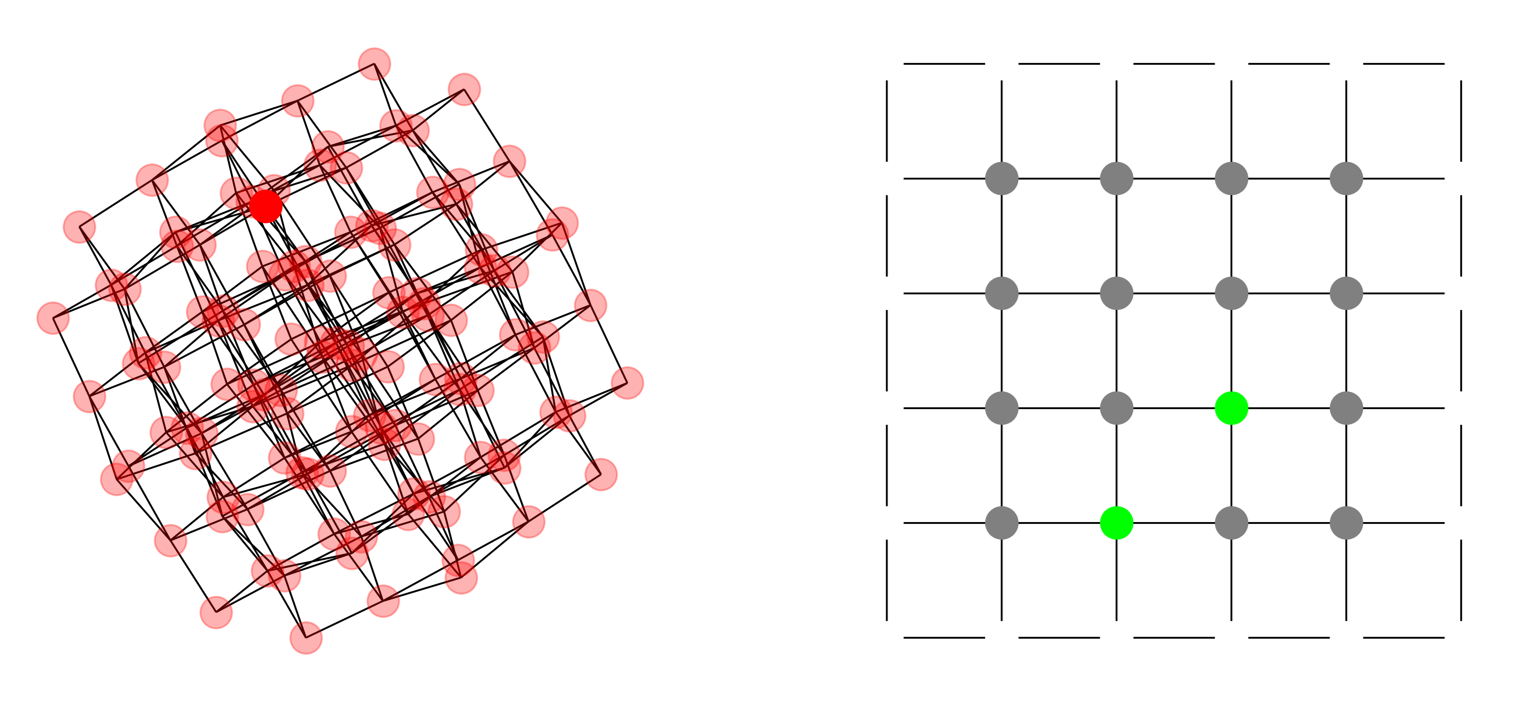
\includegraphics[width=1\textwidth]{box-4x4-2.PNG}
\end{center}
\end{posterbox}


\begin{posterbox}[name=futureresearch,column=4,below=scsofgrids]{Future Research}
We are currently exploring patterns and theoretical aspects of state complexes that hold across gridworlds of arbitrary size, geometry, and labelling. For example, an upper bound for the total number of states of a gridworld without objects is $\binom{n}{k}$ where $n$ is the total number of non-\textcolor{gray}{floor} and non-wall labels and $k$ is the total number of \textcolor{green}{agent} labels. Such information may be useful to incorporate into AI algorithms or for analysis of the efficiency, accuracy, or safety of such algorithms in gridworlds.
\end{posterbox}


\begin{posterbox}[name=references,below=futureresearch,column=4,bottomaligned=message]{References}
\renewcommand{\section}[2]{} % Get rid of the default "References" section title
\nocite{*} % Insert publications even if they are not cited in the poster
\small % Reduce the font size in this block
\bibliographystyle{unsrt}
\bibliography{sample} % Use sample.bib as the bibliography file
\end{posterbox}


\end{poster}
\end{document}